\chapter{工具原型测试}
本论文研发的工具原型的主要目的是研究使用有穷自动机来辅助日志分析的可行性和有效性。
因此,工具原型测试的目的主要是对各个模块进行可行性验证性,以及各个基本模块的功能正确性。


\section{测试目的}
论文描述的原型工具的主要目的是研究基于DFA对C语言程序进行抽象后对程序运行日志进行解析,并获得错误定位的可行性。因此,对本工具原型原型的测试主要围绕工具原型基本功能的正确性,以及原理的可行性进行验证。

论文设计了一些C语言代码样例来测试本工具原型的基本功能。这些C语言程序包括了各种类型的语句和函数调用,基本验证了工具原型能够为这些语言结构生成正确的抽象语法树,同时也测试工具原型能够为这些结构生成正确的有穷自动机。论文还通过不同完备程度的日志信息,来探究通过日志完备程度对分析获得的运行信息的完整度。

为了能够更好地检查工具原型的各个步骤的中间输出结果,以确定这些输出符合预期,作者为各个中间结果设计了可视化表示功能,以便更好地检查工具原型的功能。

当工具原型在分析源代码后得到一个有穷自动机后,使用该自动机对日志记录序列进行分析,得到相关的信息。
论文还进一步讨论了这些信息如何帮助开发人员在实际运用中更好地了解程序的运行情况,如运行成功时的具体运行路径;运行失败时对日志的识别以及提取错误发生时的调用栈内容等。同时还探讨了后续的工具开发中如何将这些分析过程自动化。

\section{测试内容}
用于测试的C语言程序包含了for,while,switch,if等常见语句和结构,以及这些语句、结构之间的不同嵌套关系,以测试工具原型是否能正确处理不同的程序结构。
此外,工具原型在适当的位置插入了log函数,用于模拟日志函数。

首先,工具原型调用Clang的cindex模块,获取源文件的翻译单元(AST的根节点),接着调用traverse函数从根节点开始、通过前序遍历的方式遍历整个AST树。为了更好地检测生成的AST树的正确性,工具原型还实现了将AST的树形结构打印出来的功能。图\ref{fig:testAST}显示了抽象语法树的一个片段。通过检查输出的抽象语法树,表明该模块的功能正确。
\begin{figure}[htbp]
	\centering	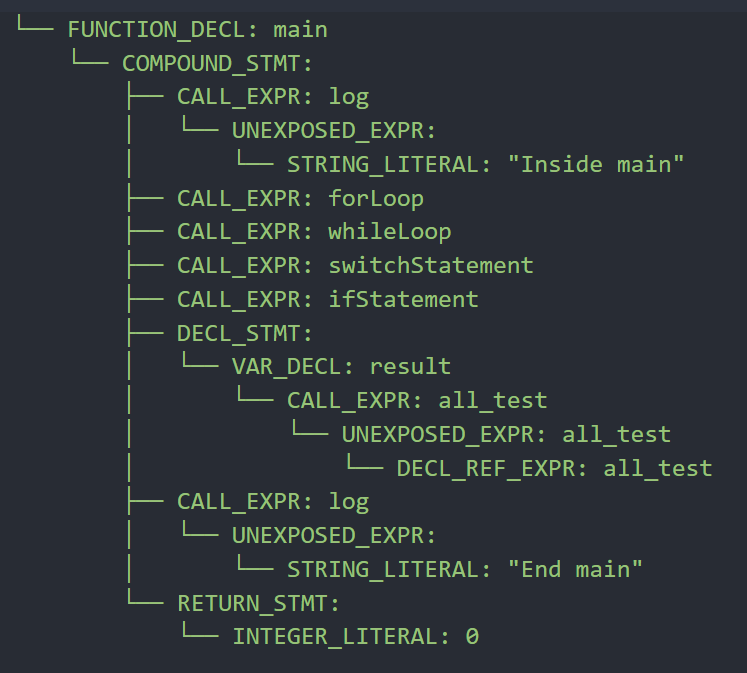
\includegraphics[width=0.7\textwidth]{pictures/testAST.png}
	\caption{AST的树形结构}
	\label{fig:testAST}
\end{figure}


然后,工具原型将通过递归的方式为整棵抽象语法树生成生成Automaton类的对象,即不确定的有穷自动机。图\ref{fig:switch语句的NFA片段}中显示了一个switch语句对应的部分自动机。
该自动机的转换中包含了一些标签。这些标签一方面可以帮助测试人员了解源代码和自动机之间的对应关系,更好地判断得到的自动机是否正确;另一方面,这些标签包含了较多的信息,有助于将来扩展工具原型的功能。

通过对生成的NFA的检查,可以确定工具原型的NFA生成模块的功能正确。

\begin{figure}[ht]
	\centering
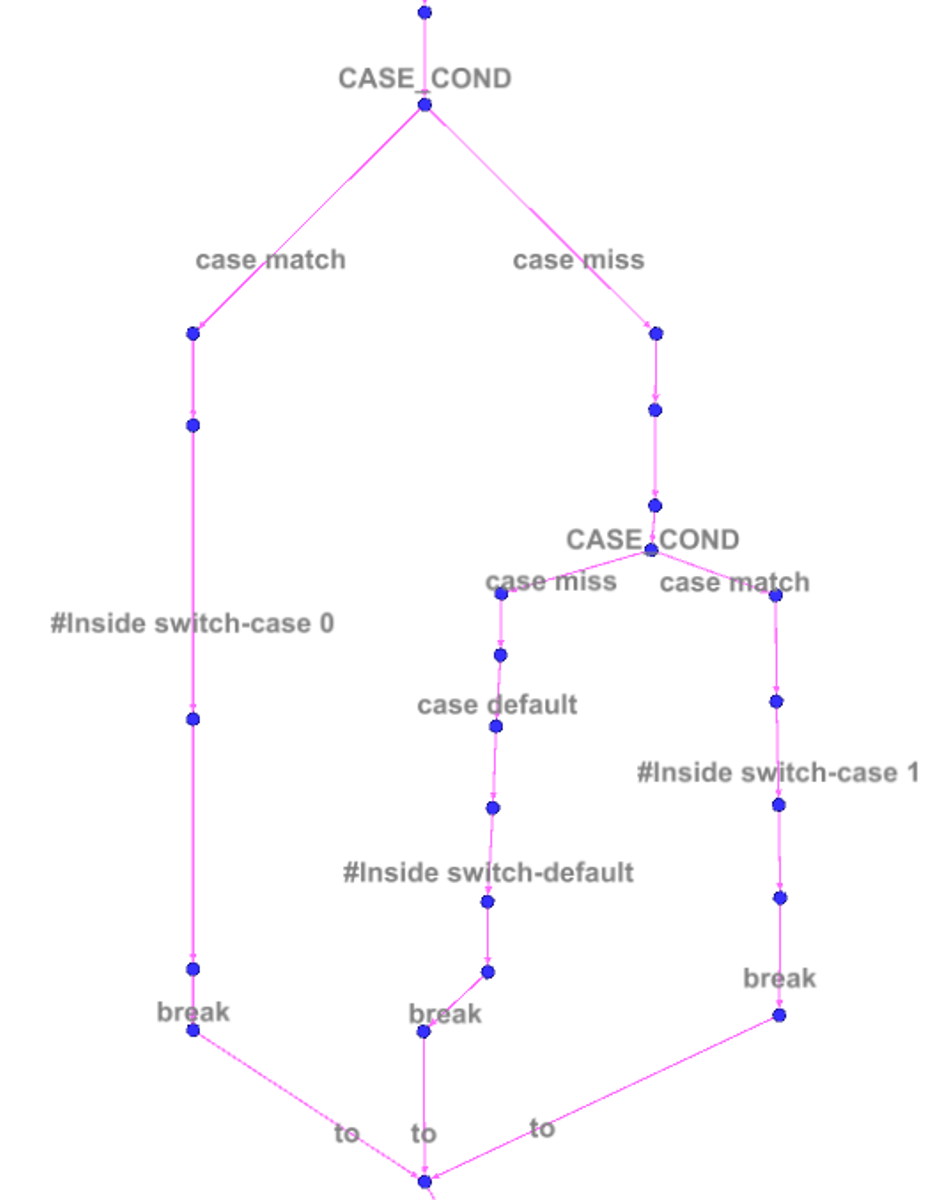
\includegraphics[width=0.7\textwidth]{pictures/switch语句的NFA片段.png}
	\caption{switch语句的NFA片段}
	\label{fig:switch语句的NFA片段}
\end{figure}

因为当前的工具原型仅考虑对日志记录的分析,因此工具原型将会从前面得到的NFA中消除无用的信息,在NFA的边的标签上仅仅保留和日志相关的信息。图\ref{fig:switch语句的NFA片段}中显示的NFA中,以“\#”开头的边上的标签对应于日志记录,因此将被保留下来,其它的标签将被消除以简化自动机。

最后,工具原型运用子集构造算法,将只保留日志函数作为输入的NFA转化为DFA。
这将自动地把一些日志无关的自动机状态和转换简化,只保留作者所关心的日志信息和它们之间的连边关系。作者测试了生成的DFA能否正确反映C语言程序的日志记录次序。也就是说,在C语言程序运行并输出日志时,所输出的日志序列必须按照DFA上的某一条路径顺序进行。测试时,首先以不同的输入数据运行C语言程序,得到不同的日志序列,然后检查这些序列是否都和DFA中的某条路径对应。这些测试表明,工具原型生成的DFA能够正确地反映C语言程序的日志记录次序。

\subsubsection{使用DFA图对日志记录的分析}

在待测试程序正常运行至结束的情况下,将会得到一个记录日志函数输出的日志记录文件。这个日志记录文件是一个由多条日志函数的输入参数组成的序列,而日志序列的顺序则是按照C语言程序调用日志函数的顺序排列。

\begin{figure}[htbp]
	\centering
	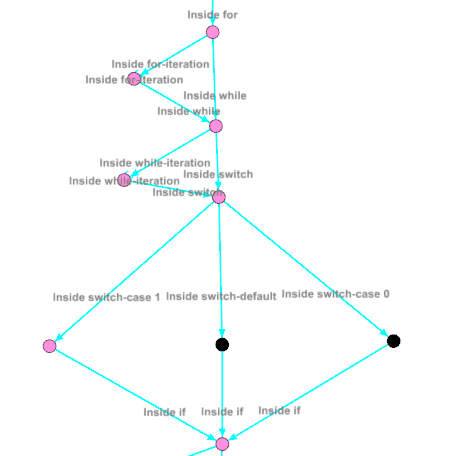
\includegraphics[width=0.7\textwidth]{pictures/正常日志分析(片段).png}
	\caption{日志分析的可视化}
	\label{fig:日志分析的可视化}
\end{figure}

作者可以使用工具原型生成的DFA(确定性有限自动机)对这段日志记录进行分析,并得到一张描述DFA运行状态的有向图(如图\ref{fig:日志分析的可视化}所示)。图中的节点和边分别代表了DFA的状态和转移。其中粉色的状态表示在分析过程中经过的状态,而黑色状态表示在分析过程中没有经过这个状态。

根据生成DFA的子集构造法的原理,图\ref{fig:日志分析的可视化}中的DFA的每一个状态节点实际上对应于多个原NFA(非确定性有限自动机)的状态节点集合,而这些原NFA状态节点是由不同语句生成的自动机的状态。


在C语言程序的实际运行中,其控制流将沿着一条全是粉色状态的路径运行。这些粉色节点代表的是语句自动机的状态合集,即程序在运行过程中可能经过的语句位置。相反,黑色节点代表的是程序在运行过程中不可能经过的语句位置。在测试中,作者可以根据这些信息直观地判断程序的运行路径。




\subsubsection{使用DFA图进行错误定位}
\emph {在开始对带有正常完备程度的日志函数的C语言程序进行错误定位之前,作者先假设一种源文件中日志函数插入较少的情况并进行分析,并解释不宜采用这种类型的日志的原因。}
\begin{figure}[htbp]
	\centering
	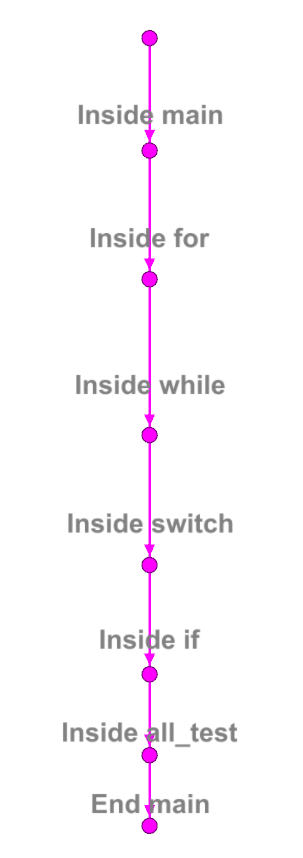
\includegraphics[width=0.25\textwidth]{pictures/不完备日志下的输出.png}
	\caption{不完备日志分析}
	\label{fig:不完备日志分析}
\end{figure}

\emph {假设当作者只对每个函数的头部插入一个日志函数时,工具原型输出的DFA图将会非常简单,如图\ref{fig:不完备日志分析}。只凭借这些信息,作者只能初略的了解程序运行时以什么样的顺序调用了哪些函数,而无法得知程序在函数内部运行的情况,如在if中选择了哪一分支,在switch中匹配了哪些case,这种信息的缺失将影响对C语言程序的错误定位的精确程度,例如C语言程序在函数A的switch语句的某一个case语句内发生了段错误,但根据得到的DFA图,作者只能确定程序在函数A内发生了错误,无法定位到具体语句。}

\emph{总之,工具原型最终生成的DFA很大程度上由C语言程序中日志记录的完备程度决定,在实际的使用中,一方面应当尽可能在程序关键位置插入合理清晰的日志,另一方面也要避免过多不必要的日志导致生成的日志记录文件过于复杂,从而导致工具原型运行缓慢。}\\

除了正常运行至结束下的日志分析,工具原型也支持对不完整日志记录的分析,以应对程序突然崩溃的情况。
在这种情况下,当作者以不完整日志记录文件为输入,同样地使用工具原型生成的 DFA 进行分析时,也将得到类似图\ref{fig:日志分析的可视化}的DFA图,但是节点的颜色分布有所不同。换言之,粉色节点组成的路径将不会到达程序的结尾。

例如,假设通过观察工具原型生成的DFA图,作者发现,C语言程序在选择了switch语句中的case1分支后,经过输出为\emph{“Inside if”}的日志函数(该日志函数位于if语句的开头)之后便停止了。这说明很有可能C语言程序在if函数中的某个环节时发生了崩溃。如此一来,便能够定位到程序运行发生错误时的具体位置。

\begin{comment}
\subsubsection{对于日志记录模块发生错误的分析}
\textcolor{red}{这一小节不需要了,因为不在作者考虑的范围内}
最后,在实际的程序测试运行中,除了C语言程序本身,日志函数或者日志记录也存在出错的可能,所以工具原型也提供了针对这类错误的分析。

当日志有非法输入时,即出现了不属于自动机的合法输入集合中的字符(日志记录),工具原型会输出:\emph{illgal input:+“那一条非法的日志记录”}。这种情况说明,在工具原型对C语言程序分析时,这一条非法的日志函数没有被扫描到;或着,有其他的程序,错误地向该日志记录文件中输入了其他内容。

当日志存在非法序列(如在日志记录中,存在从一条日志A直接跳到另一条日志B的情况,但是从工具原型生成的DFA图中,却无法找到这样的路径)时,工具原型会输出:\emph{error log!}。这种情况下只能说明,在程序测试中,负责日志记录的模块在调用两条日志函数之间突然失效。
\end{comment}

\section{本章小结}
本章节对工具原型的主要功能进行了验证和评估,测试内容包括 AST 的生成、NFA 和 DFA 的构建,以及工具原型在实际日志定位任务中的表现。通过测试案例,文章展示了工具原型的准确性和效率,并证明了所设计工具在日志解析和错误定位中的有效性。


